\documentclass[twoside]{book}

% Packages required by doxygen
\usepackage{fixltx2e}
\usepackage{calc}
\usepackage{doxygen}
\usepackage[export]{adjustbox} % also loads graphicx
\usepackage{graphicx}
\usepackage[utf8]{inputenc}
\usepackage{makeidx}
\usepackage{multicol}
\usepackage{multirow}
\PassOptionsToPackage{warn}{textcomp}
\usepackage{textcomp}
\usepackage[nointegrals]{wasysym}
\usepackage[table]{xcolor}

% Font selection
\usepackage[T1]{fontenc}
\usepackage[scaled=.90]{helvet}
\usepackage{courier}
\usepackage{amssymb}
\usepackage{sectsty}
\renewcommand{\familydefault}{\sfdefault}
\allsectionsfont{%
  \fontseries{bc}\selectfont%
  \color{darkgray}%
}
\renewcommand{\DoxyLabelFont}{%
  \fontseries{bc}\selectfont%
  \color{darkgray}%
}
\newcommand{\+}{\discretionary{\mbox{\scriptsize$\hookleftarrow$}}{}{}}

% Page & text layout
\usepackage{geometry}
\geometry{%
  a4paper,%
  top=2.5cm,%
  bottom=2.5cm,%
  left=2.5cm,%
  right=2.5cm%
}
\tolerance=750
\hfuzz=15pt
\hbadness=750
\setlength{\emergencystretch}{15pt}
\setlength{\parindent}{0cm}
\setlength{\parskip}{3ex plus 2ex minus 2ex}
\makeatletter
\renewcommand{\paragraph}{%
  \@startsection{paragraph}{4}{0ex}{-1.0ex}{1.0ex}{%
    \normalfont\normalsize\bfseries\SS@parafont%
  }%
}
\renewcommand{\subparagraph}{%
  \@startsection{subparagraph}{5}{0ex}{-1.0ex}{1.0ex}{%
    \normalfont\normalsize\bfseries\SS@subparafont%
  }%
}
\makeatother

% Headers & footers
\usepackage{fancyhdr}
\pagestyle{fancyplain}
\fancyhead[LE]{\fancyplain{}{\bfseries\thepage}}
\fancyhead[CE]{\fancyplain{}{}}
\fancyhead[RE]{\fancyplain{}{\bfseries\leftmark}}
\fancyhead[LO]{\fancyplain{}{\bfseries\rightmark}}
\fancyhead[CO]{\fancyplain{}{}}
\fancyhead[RO]{\fancyplain{}{\bfseries\thepage}}
\fancyfoot[LE]{\fancyplain{}{}}
\fancyfoot[CE]{\fancyplain{}{}}
\fancyfoot[RE]{\fancyplain{}{\bfseries\scriptsize Generated by Doxygen }}
\fancyfoot[LO]{\fancyplain{}{\bfseries\scriptsize Generated by Doxygen }}
\fancyfoot[CO]{\fancyplain{}{}}
\fancyfoot[RO]{\fancyplain{}{}}
\renewcommand{\footrulewidth}{0.4pt}
\renewcommand{\chaptermark}[1]{%
  \markboth{#1}{}%
}
\renewcommand{\sectionmark}[1]{%
  \markright{\thesection\ #1}%
}

% Indices & bibliography
\usepackage{natbib}
\usepackage[titles]{tocloft}
\setcounter{tocdepth}{3}
\setcounter{secnumdepth}{5}
\makeindex

% Hyperlinks (required, but should be loaded last)
\usepackage{ifpdf}
\ifpdf
  \usepackage[pdftex,pagebackref=true]{hyperref}
\else
  \usepackage[ps2pdf,pagebackref=true]{hyperref}
\fi
\hypersetup{%
  colorlinks=true,%
  linkcolor=blue,%
  citecolor=blue,%
  unicode%
}

% Custom commands
\newcommand{\clearemptydoublepage}{%
  \newpage{\pagestyle{empty}\cleardoublepage}%
}

\usepackage{caption}
\captionsetup{labelsep=space,justification=centering,font={bf},singlelinecheck=off,skip=4pt,position=top}

%===== C O N T E N T S =====

\begin{document}

% Titlepage & ToC
\hypersetup{pageanchor=false,
             bookmarksnumbered=true,
             pdfencoding=unicode
            }
\pagenumbering{alph}
\begin{titlepage}
\vspace*{7cm}
\begin{center}%
{\Large D\+C\+A1202\+A\+V03B }\\
\vspace*{1cm}
{\large Generated by Doxygen 1.8.14}\\
\end{center}
\end{titlepage}
\clearemptydoublepage
\pagenumbering{roman}
\tableofcontents
\clearemptydoublepage
\pagenumbering{arabic}
\hypersetup{pageanchor=true}

%--- Begin generated contents ---
\chapter{Hierarchical Index}
\section{Class Hierarchy}
This inheritance list is sorted roughly, but not completely, alphabetically\+:\begin{DoxyCompactList}
\item Q\+Main\+Window\begin{DoxyCompactList}
\item \contentsline{section}{Main\+Window}{\pageref{class_main_window}}{}
\end{DoxyCompactList}
\item Q\+Widget\begin{DoxyCompactList}
\item \contentsline{section}{Plotter}{\pageref{class_plotter}}{}
\end{DoxyCompactList}
\end{DoxyCompactList}

\chapter{Class Index}
\section{Class List}
Here are the classes, structs, unions and interfaces with brief descriptions\+:\begin{DoxyCompactList}
\item\contentsline{section}{\mbox{\hyperlink{class_main_window}{Main\+Window}} }{\pageref{class_main_window}}{}
\item\contentsline{section}{\mbox{\hyperlink{class_plotter}{Plotter}} \\*Esta é uma classe criada junto a uma interface gráfica do Qt para receber dados de um servidor e criar um gráfico com os valores recebidos. Ela é herdeira de Q\+Main\+Window }{\pageref{class_plotter}}{}
\end{DoxyCompactList}

\chapter{Class Documentation}
\hypertarget{class_main_window}{}\section{Main\+Window Class Reference}
\label{class_main_window}\index{Main\+Window@{Main\+Window}}
Inheritance diagram for Main\+Window\+:\begin{figure}[H]
\begin{center}
\leavevmode
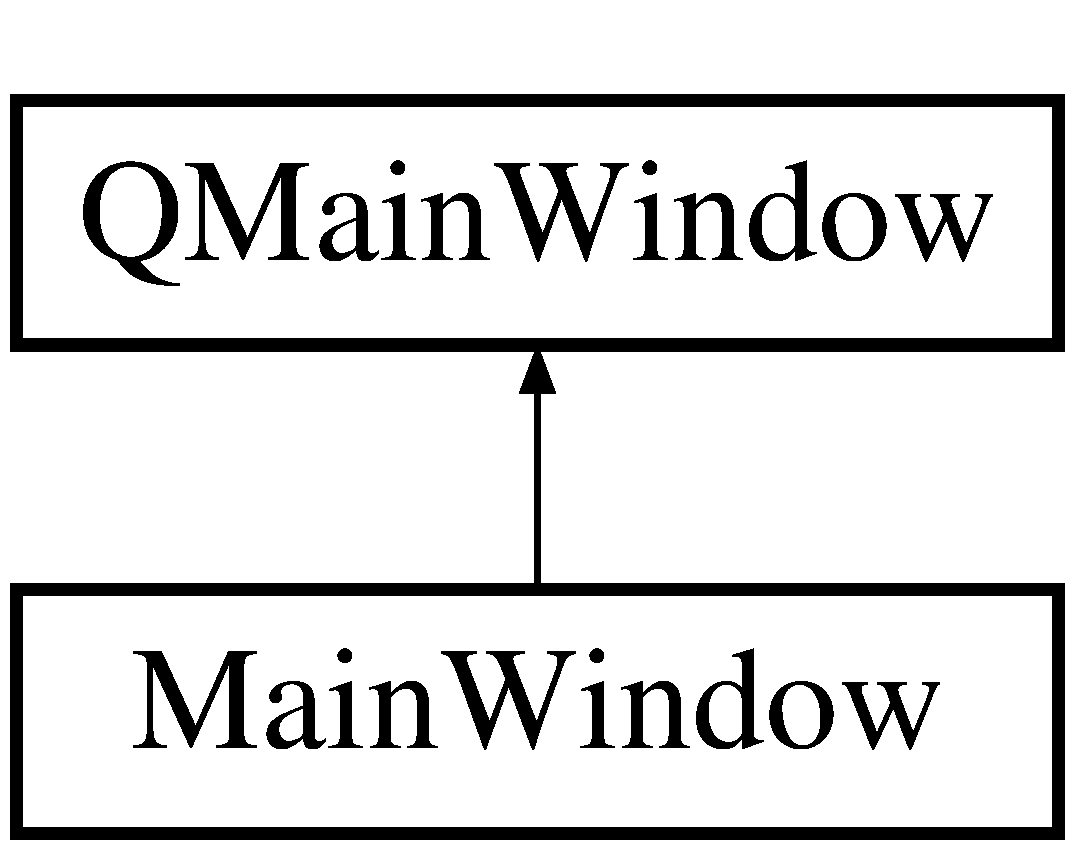
\includegraphics[height=2.000000cm]{class_main_window}
\end{center}
\end{figure}
\subsection*{Public Slots}
\begin{DoxyCompactItemize}
\item 
\mbox{\Hypertarget{class_main_window_a4a2ddf4cf2ec8e240cc340416b1df792}\label{class_main_window_a4a2ddf4cf2ec8e240cc340416b1df792}} 
void {\bfseries get\+Data} ()
\item 
\mbox{\Hypertarget{class_main_window_a66885589d165c59dc8cb39d2b005959a}\label{class_main_window_a66885589d165c59dc8cb39d2b005959a}} 
void {\bfseries addip} ()
\item 
\mbox{\Hypertarget{class_main_window_a5a8e49852ff8201bc7d7974504f7b7df}\label{class_main_window_a5a8e49852ff8201bc7d7974504f7b7df}} 
void {\bfseries removeip} ()
\item 
\mbox{\Hypertarget{class_main_window_ac83bca3631082745d67f2e3297ecde3e}\label{class_main_window_ac83bca3631082745d67f2e3297ecde3e}} 
void {\bfseries set\+IP} (Q\+String \+\_\+ipaddress)
\end{DoxyCompactItemize}
\subsection*{Public Member Functions}
\begin{DoxyCompactItemize}
\item 
\mbox{\Hypertarget{class_main_window_a8b244be8b7b7db1b08de2a2acb9409db}\label{class_main_window_a8b244be8b7b7db1b08de2a2acb9409db}} 
{\bfseries Main\+Window} (Q\+Widget $\ast$parent=0)
\end{DoxyCompactItemize}


The documentation for this class was generated from the following files\+:\begin{DoxyCompactItemize}
\item 
C\+:/\+Users/\+Lucas/\+Desktop/\+Delivery/qtsupervisory-\/master/\+Qt\+Tcp\+Client\+Consumer/mainwindow.\+h\item 
C\+:/\+Users/\+Lucas/\+Desktop/\+Delivery/qtsupervisory-\/master/\+Qt\+Tcp\+Client\+Consumer/mainwindow.\+cpp\end{DoxyCompactItemize}

\hypertarget{class_plotter}{}\section{Plotter Class Reference}
\label{class_plotter}\index{Plotter@{Plotter}}


Esta é uma classe criada junto a uma interface gráfica do Qt para receber dados de um servidor e criar um gráfico com os valores recebidos. Ela é herdeira de Q\+Main\+Window.  




{\ttfamily \#include $<$plotter.\+h$>$}

Inheritance diagram for Plotter\+:\begin{figure}[H]
\begin{center}
\leavevmode
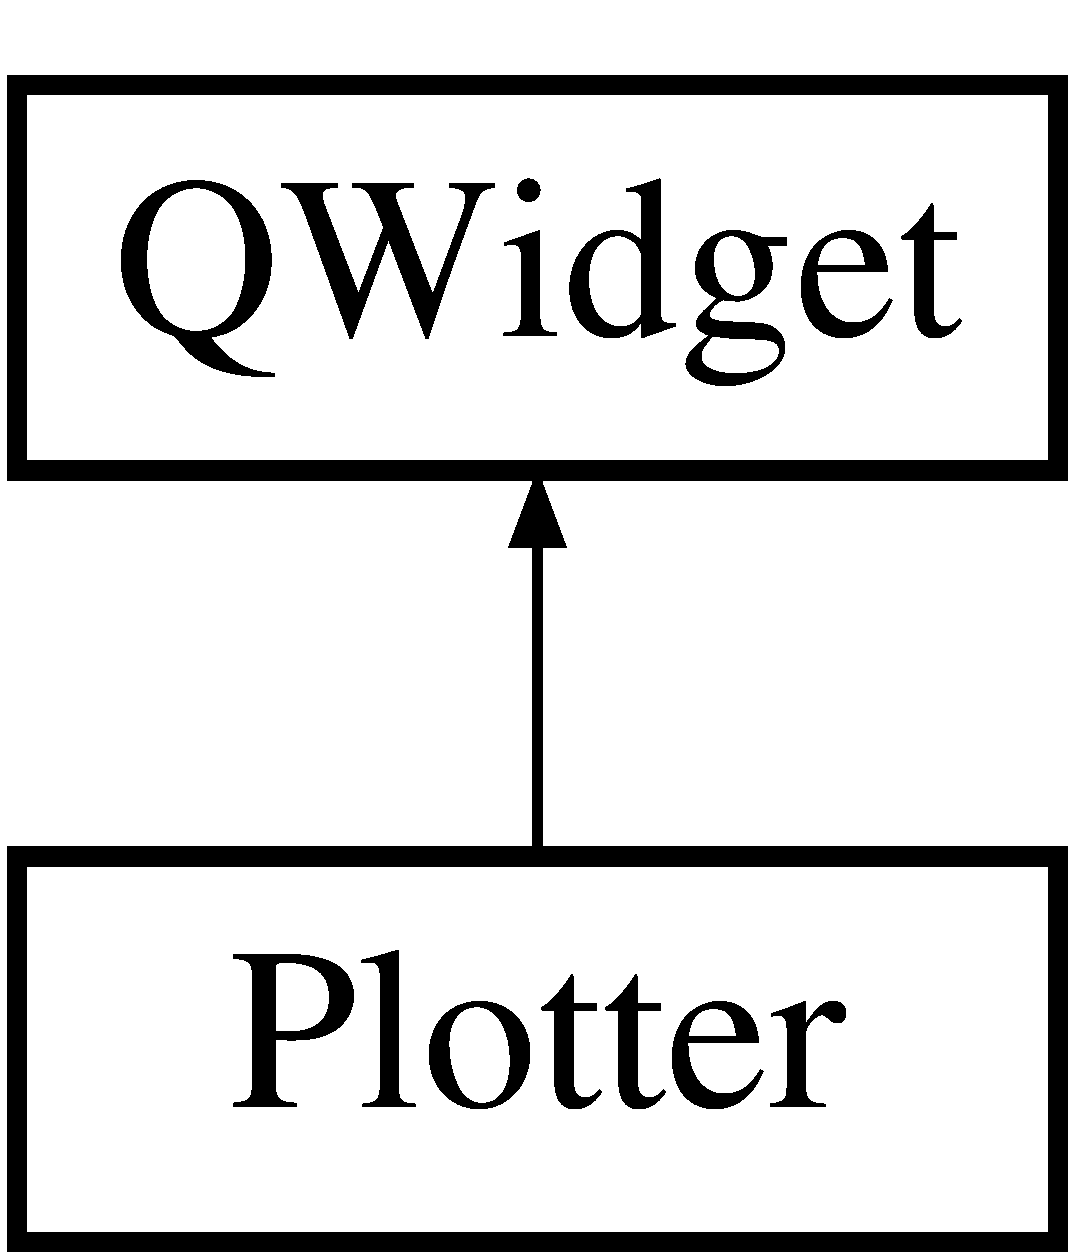
\includegraphics[height=2.000000cm]{class_plotter}
\end{center}
\end{figure}
\subsection*{Public Slots}
\begin{DoxyCompactItemize}
\item 
\mbox{\Hypertarget{class_plotter_ae42102b524033e1aa33fea567e49e406}\label{class_plotter_ae42102b524033e1aa33fea567e49e406}} 
void \mbox{\hyperlink{class_plotter_ae42102b524033e1aa33fea567e49e406}{stop\+Data}} ()
\begin{DoxyCompactList}\small\item\em Encerra o Timer. \end{DoxyCompactList}\item 
\mbox{\Hypertarget{class_plotter_a19710642f034c052eda670f75dd5e5c0}\label{class_plotter_a19710642f034c052eda670f75dd5e5c0}} 
void \mbox{\hyperlink{class_plotter_a19710642f034c052eda670f75dd5e5c0}{change\+Timing}} (int \+\_\+speed)
\begin{DoxyCompactList}\small\item\em Altera a velocidade de atualização do comando \textquotesingle{}get\textquotesingle{}. \end{DoxyCompactList}\item 
\mbox{\Hypertarget{class_plotter_a353f441c8d35b87f33b18c255757abdc}\label{class_plotter_a353f441c8d35b87f33b18c255757abdc}} 
void \mbox{\hyperlink{class_plotter_a353f441c8d35b87f33b18c255757abdc}{get\+DataB}} ()
\begin{DoxyCompactList}\small\item\em Ativa o Timer. \end{DoxyCompactList}\item 
\mbox{\Hypertarget{class_plotter_ab3f181cf97ec3e64bb3060fb0916fcfa}\label{class_plotter_ab3f181cf97ec3e64bb3060fb0916fcfa}} 
void \mbox{\hyperlink{class_plotter_ab3f181cf97ec3e64bb3060fb0916fcfa}{set\+IP}} (Q\+String \+\_\+ipaddress)
\begin{DoxyCompactList}\small\item\em Altera o endereço de IP de acordo com o que foi escrito na caixa de texto. \end{DoxyCompactList}\item 
\mbox{\Hypertarget{class_plotter_a277dfd9402cf249320f1c9f5c879e152}\label{class_plotter_a277dfd9402cf249320f1c9f5c879e152}} 
void \mbox{\hyperlink{class_plotter_a277dfd9402cf249320f1c9f5c879e152}{tcp\+Connect}} ()
\begin{DoxyCompactList}\small\item\em Inicia a conexão com o IP designado. \end{DoxyCompactList}\item 
\mbox{\Hypertarget{class_plotter_ada7a6cae3ce1cfe9966ee1a2cff891c3}\label{class_plotter_ada7a6cae3ce1cfe9966ee1a2cff891c3}} 
void \mbox{\hyperlink{class_plotter_ada7a6cae3ce1cfe9966ee1a2cff891c3}{tcp\+Disconnect}} ()
\begin{DoxyCompactList}\small\item\em Encerra a conexão com o IP designado. \end{DoxyCompactList}\end{DoxyCompactItemize}
\subsection*{Public Member Functions}
\begin{DoxyCompactItemize}
\item 
\mbox{\Hypertarget{class_plotter_a1807627530de30ae58dff3c42a823497}\label{class_plotter_a1807627530de30ae58dff3c42a823497}} 
{\bfseries Plotter} (Q\+Widget $\ast$parent=nullptr)
\item 
\mbox{\Hypertarget{class_plotter_a06477bf987646f000a8982db1352a11d}\label{class_plotter_a06477bf987646f000a8982db1352a11d}} 
void \mbox{\hyperlink{class_plotter_a06477bf987646f000a8982db1352a11d}{paint\+Event}} (Q\+Paint\+Event $\ast$event)
\begin{DoxyCompactList}\small\item\em É usada para criar o gráfico. \end{DoxyCompactList}\item 
\mbox{\Hypertarget{class_plotter_a63aa82ff02f2ff644403dfa4575c439b}\label{class_plotter_a63aa82ff02f2ff644403dfa4575c439b}} 
void \mbox{\hyperlink{class_plotter_a63aa82ff02f2ff644403dfa4575c439b}{timer\+Event}} (Q\+Timer\+Event $\ast$event)
\begin{DoxyCompactList}\small\item\em É usada para ativar a coleta dos dados e criação do gráfico. \end{DoxyCompactList}\end{DoxyCompactItemize}


\subsection{Detailed Description}
Esta é uma classe criada junto a uma interface gráfica do Qt para receber dados de um servidor e criar um gráfico com os valores recebidos. Ela é herdeira de Q\+Main\+Window. 

The documentation for this class was generated from the following files\+:\begin{DoxyCompactItemize}
\item 
C\+:/\+Users/\+Lucas/\+Desktop/\+Delivery/qtsupervisory-\/master/\+Qt\+Tcp\+Client\+Consumer/plotter.\+h\item 
C\+:/\+Users/\+Lucas/\+Desktop/\+Delivery/qtsupervisory-\/master/\+Qt\+Tcp\+Client\+Consumer/plotter.\+cpp\end{DoxyCompactItemize}

%--- End generated contents ---

% Index
\backmatter
\newpage
\phantomsection
\clearemptydoublepage
\addcontentsline{toc}{chapter}{Index}
\printindex

\end{document}
